\documentclass[tikz,border=2pt]{standalone}
\usepackage{pgfplots}
\pgfplotsset{compat=1.18}
\usetikzlibrary{positioning}
\usepackage{helvet}
\renewcommand{\familydefault}{\sfdefault}
\definecolor{ieeecolor}{HTML}{042C53}
\definecolor{jrnlcolor}{HTML}{378ADD}
\definecolor{othercolor}{HTML}{B4B2A9}
\definecolor{confcolor}{HTML}{D98B3F}
\begin{document}
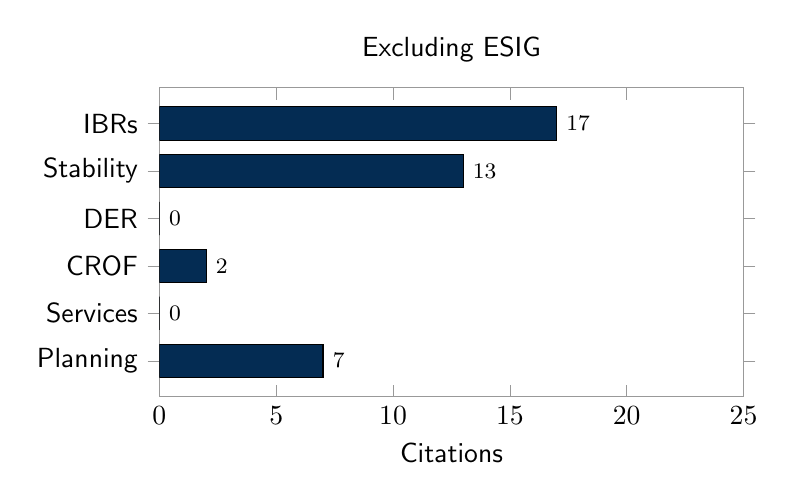
\begin{tikzpicture}
\begin{axis}[
    xbar, bar width=12pt,
    width=9cm, height=5.5cm,
    symbolic y coords={IBRs,Stability,DER,CROF,Services,Planning},
    ytick=data,
    y dir=reverse,
    xlabel={Citations},
    xmin=0, xmax=25,
    axis line style={color=black!40},
    tick style={color=black!40},
    enlarge y limits=0.15,
    nodes near coords, every node near coord/.append style={font=\footnotesize, anchor=west},
    title={Excluding ESIG},
]
\addplot[fill=ieeecolor] coordinates {(17,IBRs) (13,Stability) (0,DER) (2,CROF) (0,Services) (7,Planning)};
\end{axis}
\end{tikzpicture}
\end{document}
